\documentclass[12pt]{article}
\usepackage[utf8]{inputenc}
\usepackage[T1]{fontenc}
\usepackage[francais]{babel}
\usepackage{layout}
\usepackage{geometry}
\usepackage{soul}
\usepackage{ulem}
\usepackage{url}
\usepackage{amsmath}
\usepackage{amssymb}
\usepackage{mathrsfs}
\usepackage{graphicx}
\usepackage{wrapfig}
\usepackage{tikz}
\usepackage{hyperref}
\usepackage{pgfplots}

\title{Présentation du projet de recherche : 
What's cooking ? Use recipe ingredients to categorize the cuisine
}
\author{Ayman \bsc{Hamzaoui} \& Julien \bsc{Delaunay}}
\date{\today} 
\pagestyle{plain}
\begin{document}
\maketitle
\newpage
\tableofcontents

\newpage
\section{Introduction}
Nous avons choisi la base de données \textit{"What's cooking ? Use recipe ingredients to categorize the cuisine"}\footnote{\url{https://www.kaggle.com/c/whats-cooking-kernels-only}} parmi les bases de données de Kaggle. Le domaine de cette base de données nous est apparu intéressant et nous avons remarqué que les données fournies semblent pouvoir être séparés et ainsi analysées avec les outils appris en cours.

\section{Les données}
Les données fournies par Kaggle sont sous la forme de deux documents json. Le fichier de test et le fichier d'entraînement. Pour le fichier d'entraînement, nous avons un id de la recette, le type de cuisine pour cette recette et les ingrédients nécessaires à sa fabrication. 

\begin{wrapfigure}[8]{r}{5cm}
	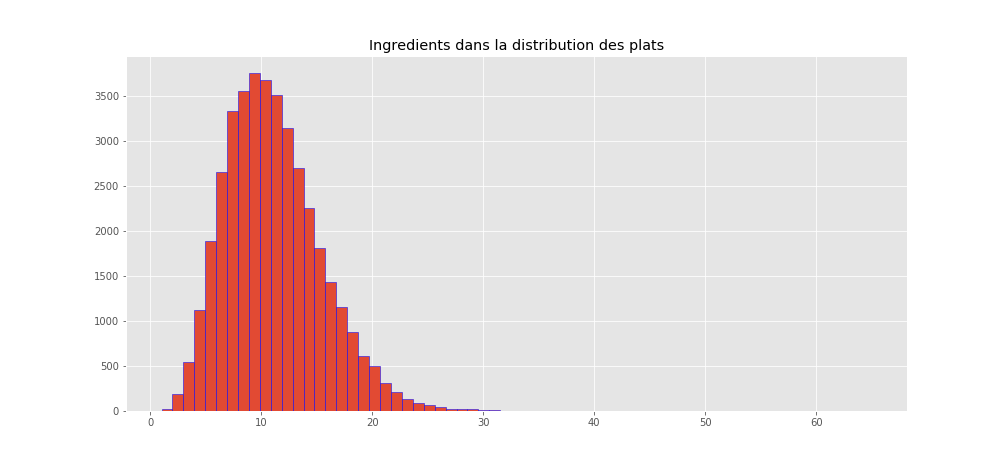
\includegraphics[width=4cm]{./repartitions_ingredients.png}
	\caption{Repartition des ingrédients}
	\label{label-image1}
\end{wrapfigure}
Nous avons effectué des recherches sur les données fournies afin d'obtenir quelques informations. Nous avons ainsi découvert que les cuisines utilisent entre 1 et 65 ingrédients par recette. Les ingrédients les plus utilisés varient en fonction des cuisines, il est donc intéressant d'observer si un modèle peut prévoir en fonction des ingrédients à quelle cuisine la recette appartient.

Nous avons observer que la base de données comportait 20 recettes, c'est donc un problème de classification avec des classes multiples. Il y a plus que 2 catégories à prédire.

\begin{wrapfigure}[5]{l}{6cm}
	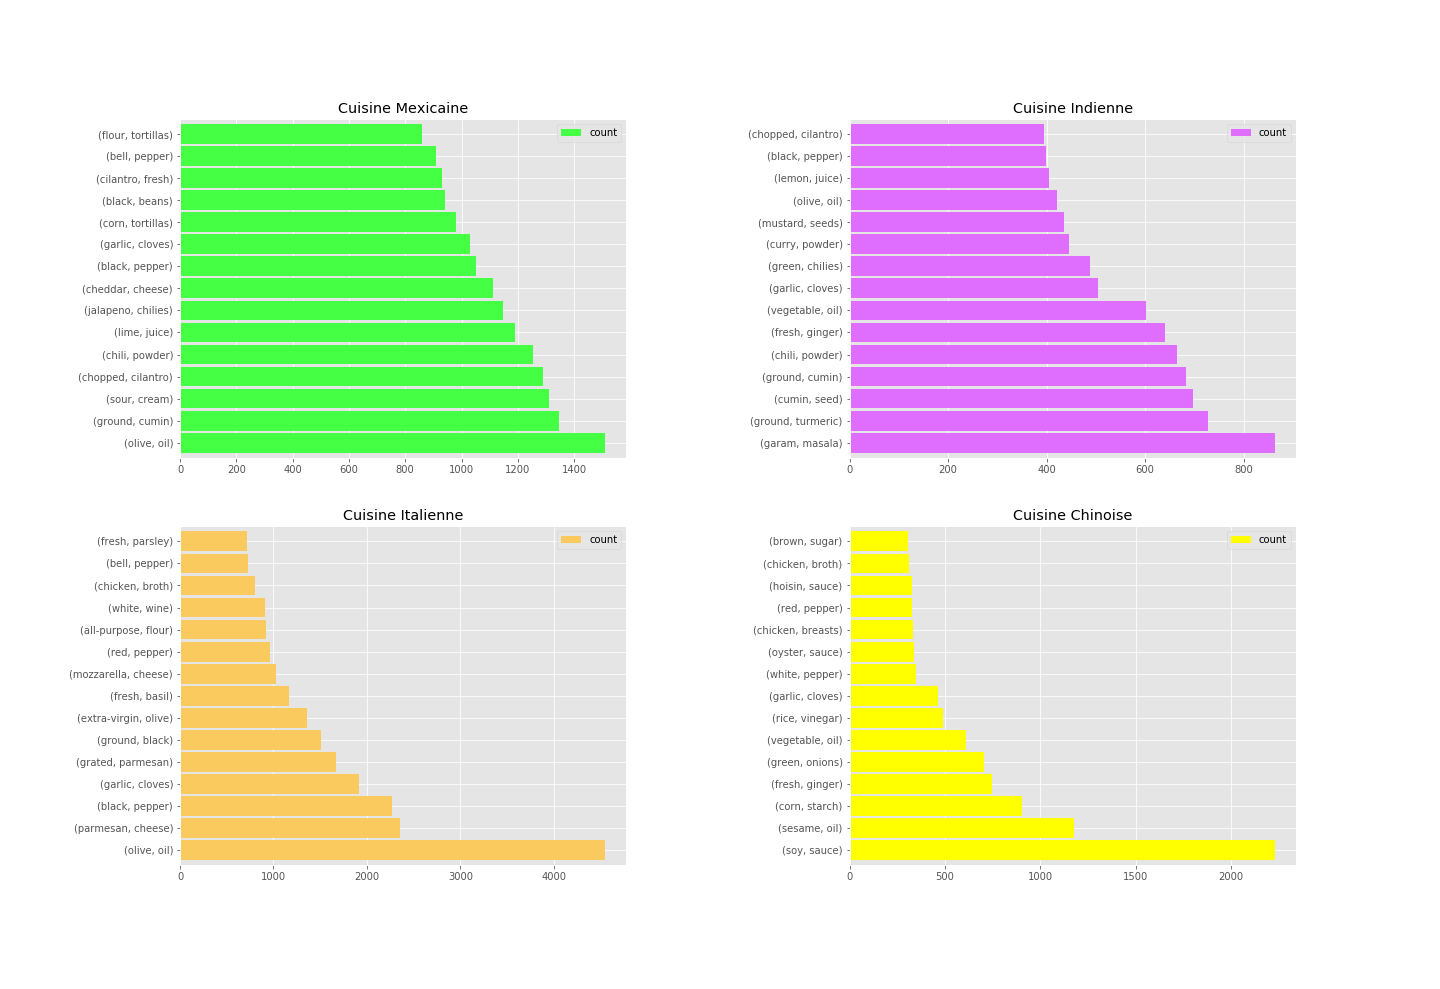
\includegraphics[width=6cm]{./exemple_differences_ingredients.png}
	\caption{Repartition des ingrédients par cuisine}
	\label{label-image2}
\end{wrapfigure}
Afin de commencer l'analyse et le traitement des données nous avons décidé de modifier le format d'entrée et transformer la liste des ingrédients sous la forme d'un tableau, avec une recette par ligne, et un ingrédients par colonne.

\newpage
\section{Traitement des données}
La partie "processing" de notre projet s'est basée sur TF-IDF. C'est une méthode de pondération qui permet d'évaluer l'importance d'un terme contenu dans un document, relativement à son ensemble. Pour ce faire, nous avons commencé par effectué une tokenisation sur le nom des ingrédients afin de bien les séparer et ne pas risquer d'erreurs par la suite dans le traitement des données. Nous avons pensé particulièrement au traitement de TF-IDF qui nécessite un token de séparation.

Par la suite, nous avons remplacer les ingrédients par des indices grâce à la fonction \textit{"label\_train\_transform"} qui peuvent ensuite être retourné sous leurs noms originels avec la fonction \textit{"label\_test\_inverseTransform"}




\section{Les méthodes utilisées\label{methodes}}
Pour le traitement des données et la recherche d'un modèle, nous avons mis en place 7 méthodes différentes à partir de scikit learn. Nous avons utilisé chaque méthode sous la forme d'une classe différente que nous avons appelée tour à tour dans notre programme principal en cherchant les meilleurs hyper-paramètres. Pour la recherche d'hyper-parametres, nous avons utilisé \textit{GridSearch.}\footnote{\url{https://scikit-learn.org/0.16/modules/generated/sklearn.grid_search.GridSearchCV.html}} Nous avons donc implémenté manuellement différentes valeurs, et \textit{GridSearch} nous aide à trouver les meilleurs hyper-paramètres. Pour chacunes de ces méthodes, dans le cas d'utilisation de \textit{GridSearch}, nous avons initialisé le nombre de processus à utiliser à 4 pour calculer le modèle plus rapidement. 

Les hyper-paramètres optimaux retournés sont localisés dans le dossier "Data/CVresult". Nous avons placé les résultats obtenus pour chaque méthode dans un fichier csv que nous avons pu ensuite soumettre sur la page de \textit{Kaggle.} 

\subsection{Les K plus proches voisins}
La méthode des K plus proches voisins\footnote{\url{https://scikit-learn.org/stable/modules/generated/sklearn.neighbors.KNeighborsClassifier.html}} que nous avons vu en cours de IFT501 nécessite la mise en place de certains arguments pour bien fonctionner : \begin{enumerate}
\item Le nombre de voisins.
\item La manière dont les poids sont distribués parmi les points d'un cluster.
\item La fonction de distance utilisée, si nous utilisons la distance Euclidienne ou la distance de Manhattan.
\end{enumerate}


\subsection{Réseaux de neuronnes}
La méthode des réseaux de neuronnes\footnote{\url{https://scikit-learn.org/stable/modules/generated/sklearn.neural_network.MLPClassifier.html\#sklearn.neural_network.MLPClassifier.fit}} de scikit learn nécessite la mise en place de certains paramètres tel que :
\begin{enumerate}
\item La taille des couches cachées.
\item La fonction d'activation.
\item Le choix du solver pour l'optimisation des poids.
\item La taille des lots (\textit{batch size.}) 
\end{enumerate}

\subsection{Machine à Vecteur de Support}
La méthode des machines à vecteur de support\footnote{\url{https://scikit-learn.org/stable/modules/generated/sklearn.svm.SVC.html}} aura de meilleurs résultat avec le bon choix de certains paramètres : 
\begin{enumerate}
\item La pénalité pour le terme d'erreur.
\item Le type de noyau qui sera évalué, tel que linéaire, rbf ou encore polynomiale.
\item La mesure du critère d'arrêt.
\item Le degré de la fonction polynomiale.
\item Le coefficient pour les noyaux rbf, polynomiale et sigmoide.
\end{enumerate}
Certains paramètres tel que le critère d'arrêt ou le maximum d'itération servent à accélerer les temps de calcul. 

\subsection{Forêt aléatoire}
La méthode des forêts aléatoires\footnote{\url{https://scikit-learn.org/stable/modules/generated/sklearn.ensemble.RandomForestClassifier.html}} nécessite la mise en place de certains paramètre pour une utilisation optimale :
\begin{enumerate}
\item Le nombre d'arbes généré dans la forêt.
\item La profondeur maximale.
\end{enumerate}

\subsection{Naive Bayes}
La méthode naive Bayes\footnote{\url{https://scikit-learn.org/stable/modules/generated/sklearn.naive_bayes.GaussianNB.html}} se base sur un paramètre principal pour construire le modèle : la variance maximale pour rendre le calcul plus stable. Nous avons donc lancé Grid Search avec deux variables différentes pour cet hyper-paramètre.

\subsection{Regression logistique}
La méthode de la regression logistique\footnote{\url{https://scikit-learn.org/stable/modules/generated/sklearn.linear_model.LogisticRegression.html}} est la méthode pour laquelle nous avons inscris le plus d'hyper paramètres.
\begin{enumerate}
\item Le critère d'arrêt.
\item La force de régularisation.
\item On décide qu'un biais doit être ajouté à la fonction de décision.
\item L'algorithme utilisé dans les problèmes d'optimisations. Etant dans un problème multi classe, nous avons le choix entre sag, saga, newton-cg et lbfgs.
\end{enumerate}

\subsection{Adaboost}
La méthode Adaboost\footnote{\url{https://scikit-learn.org/stable/modules/generated/sklearn.ensemble.AdaBoostClassifier.html}} que nous avons implémenté s'est basé sur la méthode de la regression logistique avec les paramètres optimaux que nous avons trouvés à l'aide de Grid Search. Nous avons essayé de l'implémenter avec 200 estimateurs, cependant le temps de calcul étant trop long, nous avons baissé le nombre d'estimateurs.


\newpage
\section{Les résultats}

\begin{wrapfigure}[15]{l}{6cm}
	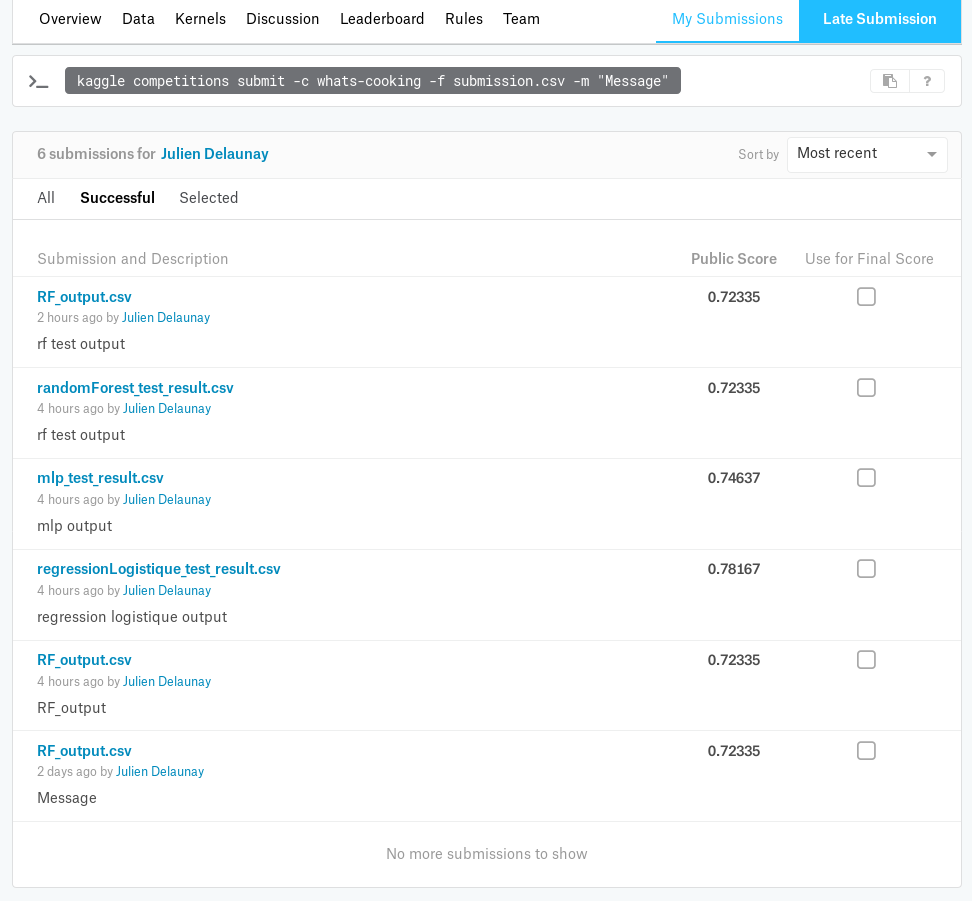
\includegraphics[width=5cm]{./soumission_kaggle.png}
	\caption{Score lors de la soumission sur Kaggle en fonction des méthodes}
\end{wrapfigure}
Nous avons donc soumis ces 7 techniques sur \textit{Kaggle} et nous avons obtenus pour 5 d'entre elles des scores supérieurs à 70\%. Les différences de score pour ces 5 méthodes ne sont pas très élévés. Cependant pour certaines, le temps de calcul est très grand et pour d'autres, beaucoup plus court.

La méthode de la forêt aléatoire à obtenu un score de 72,3\% en utilisant grid search. Pour la technique du perceptron multi couches, nous avons obtenu un score de 74,6\% tandis que la méthode de la régression logistique nous montre un score de 78,2\% et celle des machines à vecteur de support un score de 80\%.

Les méthodes pour lesquels nous avons eus de mauvais résultat sont Adaboost et naive Bayes. Nous obtenons un score de 19,3\% pour Adaboost et 33,8\% avec naive Bayes. Nous avons commencé par implémenter naive Bayes et ce mauvais résultat nous à amené à essayer une autre méthode dans l'espoir d'avoir de meilleurs résultats. C'est ainsi que nous avons implémenté une septième méthodes et au vu des résultats obtenus avec celle-ci, nous en concluons que ce sont deux méthodes qui ne sont pas adaptés aux données fournies. Les erreurs obtenues sur ces modèles sont probablement dû à la trop forte proportion de recettes italienne et indienne car nous pouvons voir sur les données de adaboost que la totalité des prévisions sont des recettes italiennes.


\section{Conclusion}
Au vu des résultats retourné par nos méthodes et des scores correspondants donnés par \textit{Kaggle}, nous pouvons conclure que la méthode la plus efficace pour ce jeu de données parmi celles que nous avons implémenté est la méthode des machines à vecteur de support. Cependant, nous avons remarqué que la méthode de la regression logistique à trouvé son modèle très rapidement et à obtenu un score de 78,2\% tandis que la méthode SVM à finit au bout de 5h. C'est une durée moyenne comparé à KNN par exemple qui a prit plus de 30h pour terminer.


\newpage
\appendix
\section{Choix du design}
\begin{wrapfigure}[10]{r}{5cm}
	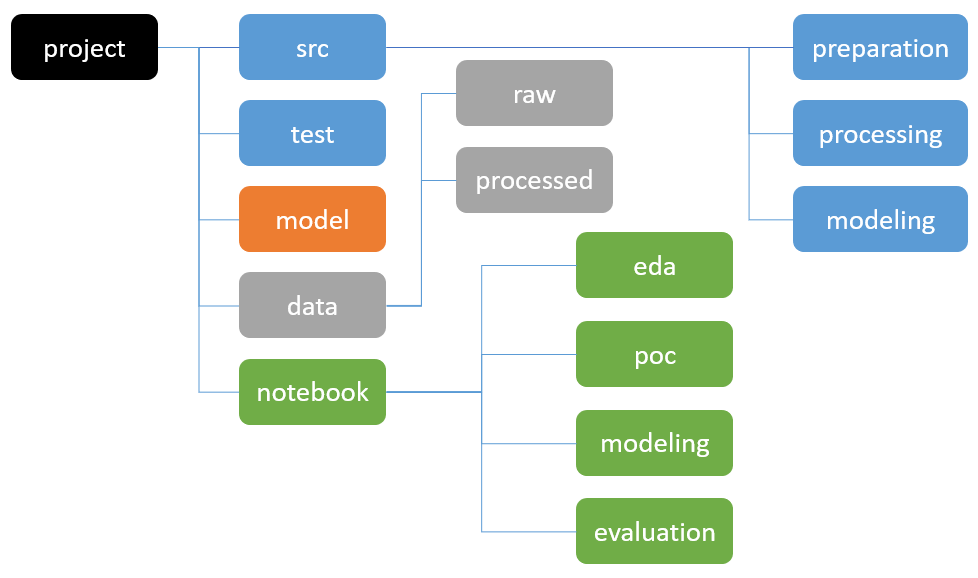
\includegraphics[width=4cm]{./projet_structure.png}
	\caption{Design d'un projet de Data Science}
\end{wrapfigure}
Pour le designe du code, nous avons utilisé ce format qui nous est inspiré de l'article écrit par Edward Ma\footnote{\url{https://goo.gl/a8cffw}}. Nous avons donc utiliser jupyter pour commencer à travailler sur les données afin de faciliter et rendre plus rapide le début du projet.\\ 
Ainsi, nous avons mis en place une partie \emph{Data} contenant les données récuperé sur \textit{Kaggle}, et les données que nous avons fournis à partir des 6 méthodes mentionnées plus haut.\ref{methodes} De plus, nous avons pu commencer par travailler sur des notebook, et donc commencer certains travaux d'une façon moins rigoureuse. 


\section{Utilisation de Git}
Nous avons mis en place un github\footnote{\url{https://github.com/hamzaouiayman/IFT_712_projet_session.git}} afin de répartir le travail et indiquer le travail restant à faire. Pour cela, nous avons crée des \textit{issues}\footnote{Tâches à effectuer avant la fin du projet} au fur et à mesure de l'avancée du projet.

\end{document}